\documentclass{article}
\usepackage{tikz}
\usetikzlibrary{matrix}

\begin{document}

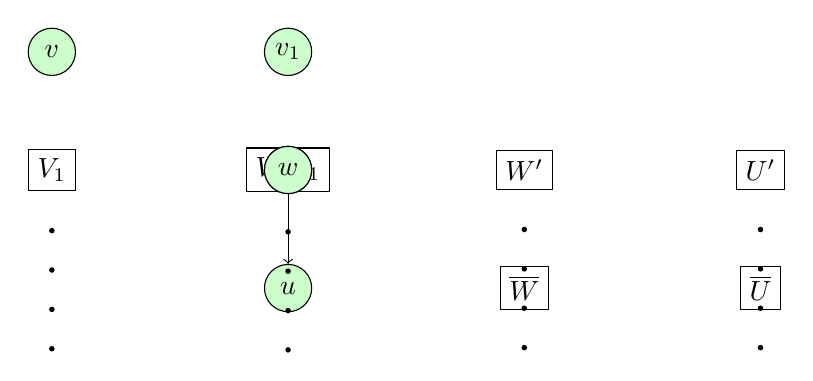
\begin{tikzpicture}[node distance=1cm]
    % Define nodes for the rectangles
    \node[draw] (V1) {$V_1$};
    \node[draw, right of=V1, node distance=3cm] (V2i-1) {$V_{2i-1}$};
    \node[draw, right of=V2i-1, node distance=3cm] (W) {$W'$};
    \node[draw, below of=W, node distance=1.5cm] (Wbar) {$\overline{W}$};
    \node[draw, right of=W, node distance=3cm] (U) {$U'$};
    \node[draw, below of=U, node distance=1.5cm] (Ubar) {$\overline{U}$};

    % Define nodes for the circles inside the rectangles
    \node[circle, draw, fill=green!20, inner sep=0pt, minimum width=6mm, label=center:$v$, above of=V1, node distance=1.5cm] (v) {};
    \node[circle, draw, fill=green!20, inner sep=0pt, minimum width=6mm, label=center:$v_1$, above of=V2i-1, node distance=1.5cm] (v1) {};
    \node[circle, draw, fill=green!20, inner sep=0pt, minimum width=6mm, label=center:$v_i$, below of=v1, node distance=1.5cm] (vi) {};
    \node[circle, draw, fill=green!20, inner sep=0pt, minimum width=6mm, label=center:$w$, below of=v1, node distance=1.5cm] (w) {};
    \node[circle, draw, fill=green!20, inner sep=0pt, minimum width=6mm, label=center:$u$, below of=w, node distance=1.5cm] (u) {};

    % Draw the dots inside the rectangles
    \foreach \x in {1,...,4} {
        \fill (V1.south) ++(0,-\x*0.5cm) circle (1pt);
        \fill (V2i-1.south) ++(0,-\x*0.5cm) circle (1pt);
        \fill (W.south) ++(0,-\x*0.5cm) circle (1pt);
        \fill (U.south) ++(0,-\x*0.5cm) circle (1pt);
    }

    % Draw the arrow between W and U
    \draw[->] (w) -- (u);
\end{tikzpicture}

\end{document}